\chapter{Introducción}

La digitalización y el desarrollo de software han comenzado a transformar el funcionamiento de las disciplinas creativas, abriendo nuevas oportunidades de optimización para el rubro del arte corporal. El diseño e implementación de plataformas a la medida permite a los artistas modernos modernizar sus flujos de trabajo tradicionales, logrando un equilibrio eficiente entre la gestión administrativa del estudio y la ejecución de su obra.\\
\indent El presente capítulo tiene como propósito describir las bases que fundamentan el trabajo realizado en esta memoria de título. Para ello, se expone inicialmente el contexto de crecimiento del rubro del tatuaje, seguido de la descripción detallada de la problemática detectada a nivel operativo y administrativo. Posteriormente, se define la propuesta de solución tecnológica, sus objetivos, los alcances que delimitan el desarrollo y, finalmente, el plan de trabajo estructurado para su ejecución.

\section{Contexto}

El presente marco teórico establece los fundamentos históricos, comerciales y socioculturales que respaldan el desarrollo de la plataforma. Para comprender la envergadura y necesidad de este proyecto, es necesario analizar la evolución del rubro del tatuaje, partiendo desde sus orígenes hasta consolidarse como una industria global, para luego conectar estas métricas en la realidad nacional y local.

El tatuaje forma parte de la historia del ser humano, siendo la evidencia más antigua el hallazgo de los restos momificados del cazador neolítico conocido como ``Ötzi'', datados hace más de 5.300 años. En civilizaciones antiguas, como la egipcia, romana y maya, la inserción de pigmentos bajo la epidermis cumplía funciones estrictamente identitarias, indicando estatus o linaje, y en otros casos, marcando a prisioneros y esclavos \cite{ballen2015}. Si bien durante gran parte de la historia occidental moderna el tatuaje estuvo estigmatizado y relegado a la criminalidad, a partir del siglo XX y XXI ha experimentado una resignificación profunda. En la actualidad, ha superado el estigma social para consolidarse como una expresión artística legítima y un medio de afirmación de la identidad y la subjetividad personal \cite{poulsen2021}.

En la actualidad, la industria del arte corporal es uno de los mercados de más rápido y constante crecimiento en el mundo. Según estimaciones globales, la industria alcanzó un valor aproximado de 2.420 millones de dólares en el año 2025, y se proyecta que ascienda a 6.220 millones de dólares para el año 2035, exhibiendo una Tasa de Crecimiento Anual Compuesta (CAGR) del 9,9 \% \cite{ide2026}. Este crecimiento exponencial está directamente impulsado por la creciente aceptación social de las modificaciones corporales, el cambio demográfico liderado por las generaciones ``Millennials'' y ``Gen Z'', y un mayor poder adquisitivo destinado a la autoexpresión \cite{ide2026}.

Esta tendencia global también se encuentra en el panorama chileno. Un estudio estadístico realizado por la consultora GfK Adimark evidenció que el 17 \% de los chilenos mayores de 15 años posee al menos un tatuaje. Dicha cifra experimenta un alza dramática al observar el segmento de adultos jóvenes (entre 25 y 34 años), donde el 38 \% de la población se encuentra tatuada. En la última década, la demanda en el país ha crecido de manera exponencial, posicionando el nivel técnico y artístico del tatuaje en Chile a la par de los mercados europeos y norteamericanos\cite{sepulveda2017}.

En un contexto local, la ciudad de Curicó no ha quedado ajena a esta explosión de demanda. El aumento sostenido de clientes ha propiciado la apertura de nuevos estudios y el establecimiento de artistas independientes en la zona que buscan ganarse un puesto en el mercado local. Por consiguiente, el desarrollo de este proyecto cobra una relevancia para el apoyo a este dinamismo local. Al dotar a los artistas de Curicó con herramientas tecnológicas, se busca potenciar su capacidad y facilitar su consolidación en un mercado en plena expansión.

\subsection{Descripción del problema}

Actualmente el trabajo de los tatuadores se encuentra muy fragmentando por las diferentes herramientas tecnológicas que se pueden utilizar al momento de realizar su trabajo, ya sea en el ámbito operativo como en lo artístico. El hecho de dividir sus labores crea dificultades para optimizar sus tareas de una forma limpia.

A continuación se detallan las problemáticas operativas y administrativas, las cuales fueron analizadas y planteadas por el señor Héctor Salazar Moya quien es un tatuador profesional de Curicó, que ha trabajado en el área durante varios años y en distintos estudios de tatuajes, por lo que tiene un conocimiento profundo de las dificultades que enfrentan los tatuadores de la actualidad.

En el ámbito operativo, uno de los mayores problemas es la previsualización del tatuaje en una zona concreta del cuerpo. Actualmente para visualizar como quedaría un boceto de un tatuaje se ocupa un elemento llamado ``stencil'', que es una guía en papel hectográfico que transfiere el diseño del papel a la piel del boceto original. El problema surge que este papel es un material que se desecha una vez utilizado, esto quiere decir que si el tatuador se equivoca en la posición que coloca el stencil tendría que repetirse de nuevo el proceso y ocupar material extra. Incluso muchas veces son los mismos clientes que cambian de opinión con respecto a la posición que les gustaría tener su tatuaje, y el hecho de que el tatuador pueda previsualizar el boceto en cualquier parte del cuerpo que considere el lugar más apropiado, le facilitaría sus decisiones artísticas y no tendría los problemas antes mencionados.

Con respecto al ámbito admnistrativo, es posible mencionar más problemáticas que viven los tatuadores para la gestión de su negocio. Para comenzar el agendamiento de las citas es uno de los principales problemas, debido a que no existe una herramienta dedicada para los tatuadores, lo que hace que la gestión de citas sea poco personalizable y haya problemas en la estructuración de tiempos del profesional. En relación a las citas, también hay problemas con los recordatorios hacia los clientes, debido a que muchos de ellos no se presentan a la hora adecuada o simplemente se olvidan de su cita el día acordado, debido a que es el tatuador el que tiene que recordar a sus clientes de forma manual el día antes de la sesión, por lo que al tener múltiples clientes esta acción se puede ver afectada por parte del tatuador.

Otro de los problemas es analizar correctamente el coste los tatuajes, si bien este precio se ve influnciado gran parte por el valor que le quiera dar el artista, analizar su costo real a partir de los materiales utilizados y el tiempo invertido en las sesiones es una labor que es dificil tenerla presente en todo momento.

Por último hay que mencionar también el problema con respecto a la gestión del inventario ya que surgen inconvenientes al momento de gastar insumos y no tener las nociones de cuanto material se va utilizando en cada sesión de trabajo y calcular también su reposición.

\begin{figure}[h]
  \centering
  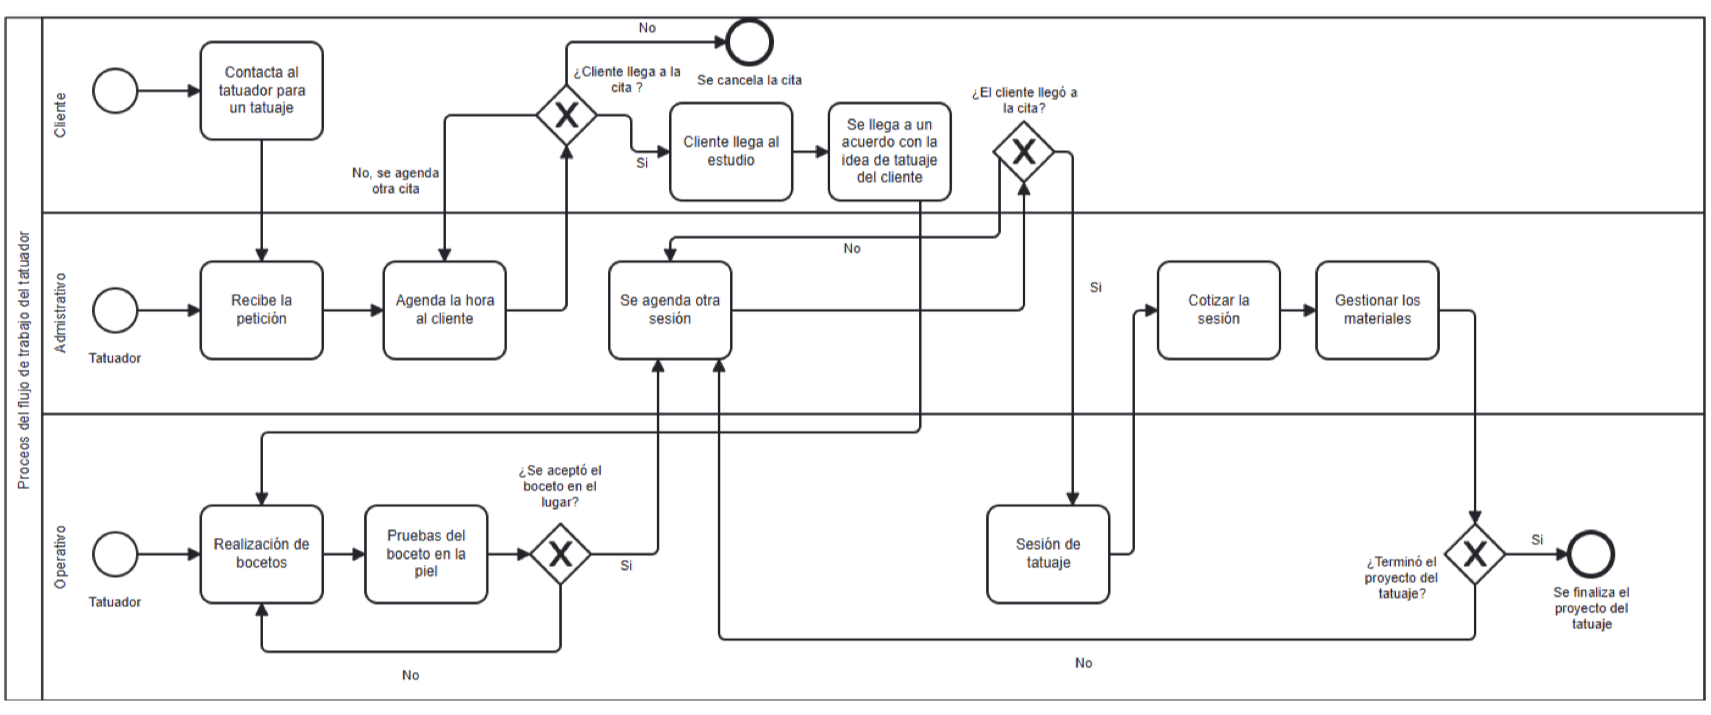
\includegraphics[width=\textwidth]{fig-1-1-bpmn}
  \caption[Modelo del proceso de negocio de un estudio de tatuajes (BPMN)]{Modelo del proceso de negocio de un estudio de tatuajes (BPMN)\cite{white2004}.}
  \label{fig:bpmn}
\end{figure}

La Figura \ref{fig:bpmn} representa el flujo del trabajo del tatuador, incluyendo su participación con el cliente, sus labores operativas y admistrativas. Esto describe la complejidad que conlleva desarrollar un proyecto de tatuaje con múltiples iteraciones, ya que, además de ser un proceso extenso, puede involucrar múltiples retrasos por parte del cliente al no poseer un recordatorio automatizado. Por otro lado los procesos que se integran en el trabajo son desarrollados en diferentes herramientas tanto admistrativamente como operativamente, lo que retrasa aún más este flujo.

\subsection{Propuesta de solución }

La solución propuesta consiste en el diseño y construcción de una plataforma web/móvil que unifique el flujo del trabajo de los artistas dedicados al arte del tatuaje, varias de sus funciones fueron creadas a partir de los requisitos de tatuador experto. El sistema considera distintos módulos como la importación y almacenamiento en la nube para la gestión de bocetos, la previsualización 3D sobre modelos anatómicos, el agendamiento de citas con recordatorios para reducir la inasistencia y retrasos de los clientes, un gestor de cotizaciones automatizadas y gestión de inventario.

Con respecto al módulo de importación y almacenamiento en la nube, este permite subir imágenes de los bocetos a la plataforma donde serán guardadas y visibles en la galería de la aplicación. Adicionalmente, el módulo contempla la generación de un enlace público asociado a la galería del tatuador, el cual puede ser compartido con clientes u otras personas interesadas para que visualicen el portafolio de diseños disponibles sin necesidad de contar con una cuenta en la plataforma.

En cuanto al módulo de previsualización 3D sobre modelos anatómicos, este permite visualizar un modelo 3D de un cuerpo humano en la plataforma gracias a un motor de renderizado, en donde los bocetos subidos son transformados para adherirse a la superficie 3D del cuerpo y desplazarse para encontrar la posición y el ángulo que el cliente prefiera.

Sobre el módulo de agendamientos de citas con recordatorios, este permite hacer agendas personalizadas, en donde se puede crear las citas a partir de los nombres de las personas a atender, en las cuales para cada perfil se puede crear una nueva sesión de tatuaje o un nuevo proyecto, donde se pueden incluir la hora de la cita, el precio de la sesión o proyecto, junto con una foto del proceso del tatuaje. Para el problema de los recordatorios se propone implementar una API que integra los mensajes de WhatsApp\cite{whatsapp}, donde se vinculan los números para enviar avisos antes y despues de la sesión del tatuaje.

El módulo de gestión de cotizaciones automatizadas, permite calcular el precio aproximado del costo del tatuaje a partir del boceto subido a la plataforma, esto se realiza mediante un algoritmo que procesa las dimensiones del boceto, junto con otros parámetros como el grosor de los trazados y colores, ya que el costo se centra en los gastos de material como agujas, tinta y otros insumos para la elaboración del tatuaje, dejando de lado valor adicional que le quiera dar el artista de acuerdo a la complejidad del diseño.

Por último, el módulo de gestión de inventario se encarga de gestionar los materiales que posea el tatuador, ya sea agujas, tintas, insumos de higiene, entre otros, los que puede a editar a su disposición y a la vez se pueden actualizar automaticamente cada vez que se haga una cotización automatizada.

En términos de factibilidad, esta solución es viable gracias a varios factores en los que incluye factibilidad técnica, operativa y económica. En el ámbito técnico, la solución se apoya en las tecnologías orientadas al desarrollo web, empleando librerías de código abierto establecidas para el renderizado 3D en el navegador e integraciones mediante protocolos estándar para las APIs de mensajería, lo que elimina la necesidad de desarrollar motores gráficos desde cero o adquirir licencias de software. Operativamente, se sustenta directamente con las necesidades reales de los tatuadores, en mayor medida dentro de la zona local, debido a que gran parte de los requerimientos son parte de las ideas del tatuador experto, que estuvo dispuesto a buscar mejoras en el flujo de su trabajo con la plataforma gracias a sus requerimientos, y es por ello que estuvo dispuesto a participar y validar prototipos y avances relacionados a la plataforma. Finalmente, la viabilidad económica se garantiza al basar la arquitectura en lenguajes de programación y gestores de bases de datos gratuitos, lo que reduce a cero los costos iniciales por licencias, mientras que los gastos de infraestructura se mantendrán al mínimo aprovechando entornos locales y capas gratuitas de servicios en la nube durante las fases de desarrollo y pruebas de concepto.

\section{Objetivos}

En esta sección se presentan el objetivo general y especifícos del proyecto.

\subsection{Objetivo general:}

Optimizar el flujo del trabajo artístico y administrativo de los tatuadores mediante una plataforma web que integre previsualización 3D, agendamiento personalizado de citas, cotizaciones automatizadas y gestión de inventario.

\vspace{\parskip}
\subsection{Objetivos específicos:}

\begin{itemize}
  \item Analizar los procesos actuales de los tatuadores, mediante entrevistas para obtener métricas a optimizar.
  \item Disminuir en al menos un 50\% el ausentismo y retrasos de los clientes a sus sesiones mediante un módulo de agendamientos de citas con recordatorios.
  \item Reducir en al menos un 40\% el tiempo empleado en el cálculo manual de costos y revisión de stock mediante un módulo de cotizaciones automatizadas y gestión de inventario.
  \item Reducir en al menos un 30\% el tiempo invertido en pruebas de tamaño y ubicación del diseño en el cliente mediante un módulo de previsualización 3D sobre modelos anatómicos.
  \item Implementar un módulo de importación y almacenamiento en la nube para la gestión de bocetos.
  \item Evaluar la calidad de la solución implementada a través de la ejecución de tests unitarios (integración), caja negra, caja blanca con cobertura de al menos 95\%.
  \item Validar el sistema mediante pruebas de aceptación con al menos un 90\% de evaluación positiva con el usuario y una evaluación de usabilidad aplicando un cuestionario SUS con un puntaje de al menos 85 puntos en escala Likert.
\end{itemize}

\section{Alcances}

En esta sección se presentan los alcances del proyecto.

\begin{itemize}
  \item En este trabajo se espera implementar el Producto Mínimo Viable (MVP) que incluye la web funcional con importación de bocetos, mapeo 3D en navegador, calculadora de costos y gestor de citas con API de mensajería.
  \item No se considera implementar un módulo que permita la creación de bocetos mediante dibujo en la plataforma.
  \item En este trabajo no se incluye la modificación avanzada de bocetos mediante Inteligencia Artificial Generativa.
  \item No se contempla implementar visualización en Realidad Aumentada (AR) sobre la piel en tiempo real, limitando la visualización al entorno 3D web.
  \item El sistema considera la importación en formato imágenes PNG, con un tamaño limitado para garantizar un rendimiento fluido para el renderizado 3D.
  \item La plataforma considera modelos 3D ya integrados (cuerpo humano, brazo, pierna, torso). No se contempla la funcionalidad de subir modelos 3D por parte del usuario.
  \item El algoritmo de cotización de tatuaje no incluye un precio que contemple el arte del tatuaje. Solo de insumos u otros gastos objetivos.
\end{itemize}

\section{Plan de trabajo}

A continuación se presenta el plan de trabajo del proyecto.

\subsection{Descripción de etapas del proyecto}

En esta sección se presentan las etapas que posee el proyecto, tareas más importantes y la cantidad de semanas de duración que implicará realizar cada etapa.

\begin{enumerate}
  \item Requerimientos (2 semanas)
  \begin{itemize}
    \item Capturar requerimientos mediante reuniones con el cliente experto.
  \end{itemize}
  \item Planificación (9 semanas)
  \begin{itemize}
    \item Creación y estimación de historias de usuario.
    \item Definición de tecnologías.
    \item Entrevista a cliente sobre métricas de objetivos específicos.
    \item Diseño de la arquitectura del sistema y del modelo de la base de datos.
    \item Diseño de interfaces (Mockups) centradas en la usabilidad móvil y web.
    \item Analizar las consideraciones de guía de desarrollo seguro.
  \end{itemize}
  \item Implementación (13 semanas)
  \begin{itemize}
    \item Configuración inicial del proyecto.
    \item Implementar módulo de autenticación de usuarios.
    \item Implementar módulo de importación y almacenamiento en la nube para la galería de bocetos.
    \item Implementar módulo de gestión de inventario.
    \item Implementar módulo de cotizaciones automatizadas conectadas al inventario.
    \item Implementar módulo de agenda de citas e integración con la API de mensajería para recordatorios.
    \item Implementar módulo de previsualización 3D sobre modelos anatómicos.
  \end{itemize}
  \item Evaluación y Validación (4 semanas)
  \begin{itemize}
    \item Ejecutar pruebas de caja blanca (unitarias).
    \item Aplicar pruebas de caja negra.
    \item Realizar marcha blanca de la aplicación con el cliente experto.
    \item Aplicar prueba de usabilidad (SUS) y evaluar la aceptación del usuario (UAT).
  \end{itemize}
  \item Conclusión (2 semanas)
  \begin{itemize}
    \item Realizar entrevista final y comparar métricas para verificar el cumplimiento de los porcentajes de optimización planteados.
    \item Realizar conclusiones y completar documento.
  \end{itemize}
\end{enumerate}

Quedando así un total de 30 semanas para el desarrollo del proyecto. Para mayor detalle de la planificación revisar la Carta Gantt anexo al documento.

\subsection{Tareas para objetivos específicos}

Para asegurar la trazabilidad entre el plan de trabajo y las metas del proyecto, se detallan las acciones que darán cumpliento a los objetivos específicos planteados:

\begin{itemize}
  \item \textbf{Análisis de los procesos actuales y obtención de métricas a optimizar:}
  \begin{itemize}
    \item \textit{Etapa 1:} Entrevistar al cliente para levantar tiempos actuales de cotización, tiempos de prueba de diseño y tasas de inasistencia.
  \end{itemize}
  \item \textbf{Reducir tiempos de cotización e inventario en un 40\%:}
  \begin{itemize}
    \item \textit{Etapa 3:} Implementar iterativamente los módulos lógicos de inventario y calculadora de costos.
    \item \textit{Etapa 5:} Comparar tiempos manuales originales versus el uso del sistema automatizado.
  \end{itemize}
  \item \textbf{Disminuir ausentismo en un 50\%:}
  \begin{itemize}
    \item \textit{Etapa 3:} Desarrollar integración con API de mensajería para envío de notificaciones 24 horas antes de la cita.
    \item \textit{Etapa 5:} Medir la variación en la asistencia registrada tras un mes de marcha blanca.
  \end{itemize}
  \item \textbf{Reducir tiempos de previsualización en un 30\%:}
  \begin{itemize}
    \item \textit{Etapa 3:} Desarrollar el módulo de previsualización 3D en la web.
    \item \textit{Etapa 5:} Cuantificar el ahorro de tiempo al evitar imprimir y posicionar stencils físicos múltiples veces.
  \end{itemize}
  \item \textbf{Validación de Usabilidad (SUS $\geq$ 85):}
  \begin{itemize}
    \item \textit{Etapa 4:} Aplicar cuestionario de Likert a los usuarios de prueba tras la fase de marcha blanca y procesar el puntaje final.
  \end{itemize}
\end{itemize}

\section{Resumen del capítulo}

En este capítulo, se dió a conocer el tema del proyecto, permitiendo comprender el contexto, el cual se centra en la transformación en el mundo del tatuaje, como su popularidad a lo largo de la historia y los métodos de trabajo. También se presenta la problemática que se poseen en el y rubro y la solución propuesta a este problema, el cual es la construcción de un sistema de un sistema que permita gestionar la mayor de procesos de un tatuador para la optimización de su flujo de trabajo.

A continuación, el Capítulo 2 detallará conceptos básicos del proyecto, tecnologías a utilizarm estado del arte y metodologías, tanto de desarrollo como de evaluación.
